%!TEX root = ../../main.tex
\section{Metoder}

I dette projekt er der blevet brugt følende arbejdsmetoder:
\begin{itemize}
	\item V-Modellen
	\item SCRUM (afskygning)
	
\end{itemize}

\subsection{V-Modellen}

V-Modellen, som er en udviklingsmodel, er blevet brugt i dette projekt til at lave test løbende. Da der laves test sideløbende sikres der at systemet virker efter hensigten. På figur \ref{VModel} kan V-Modellen ses.

\begin{figure}[H]
	\centering
	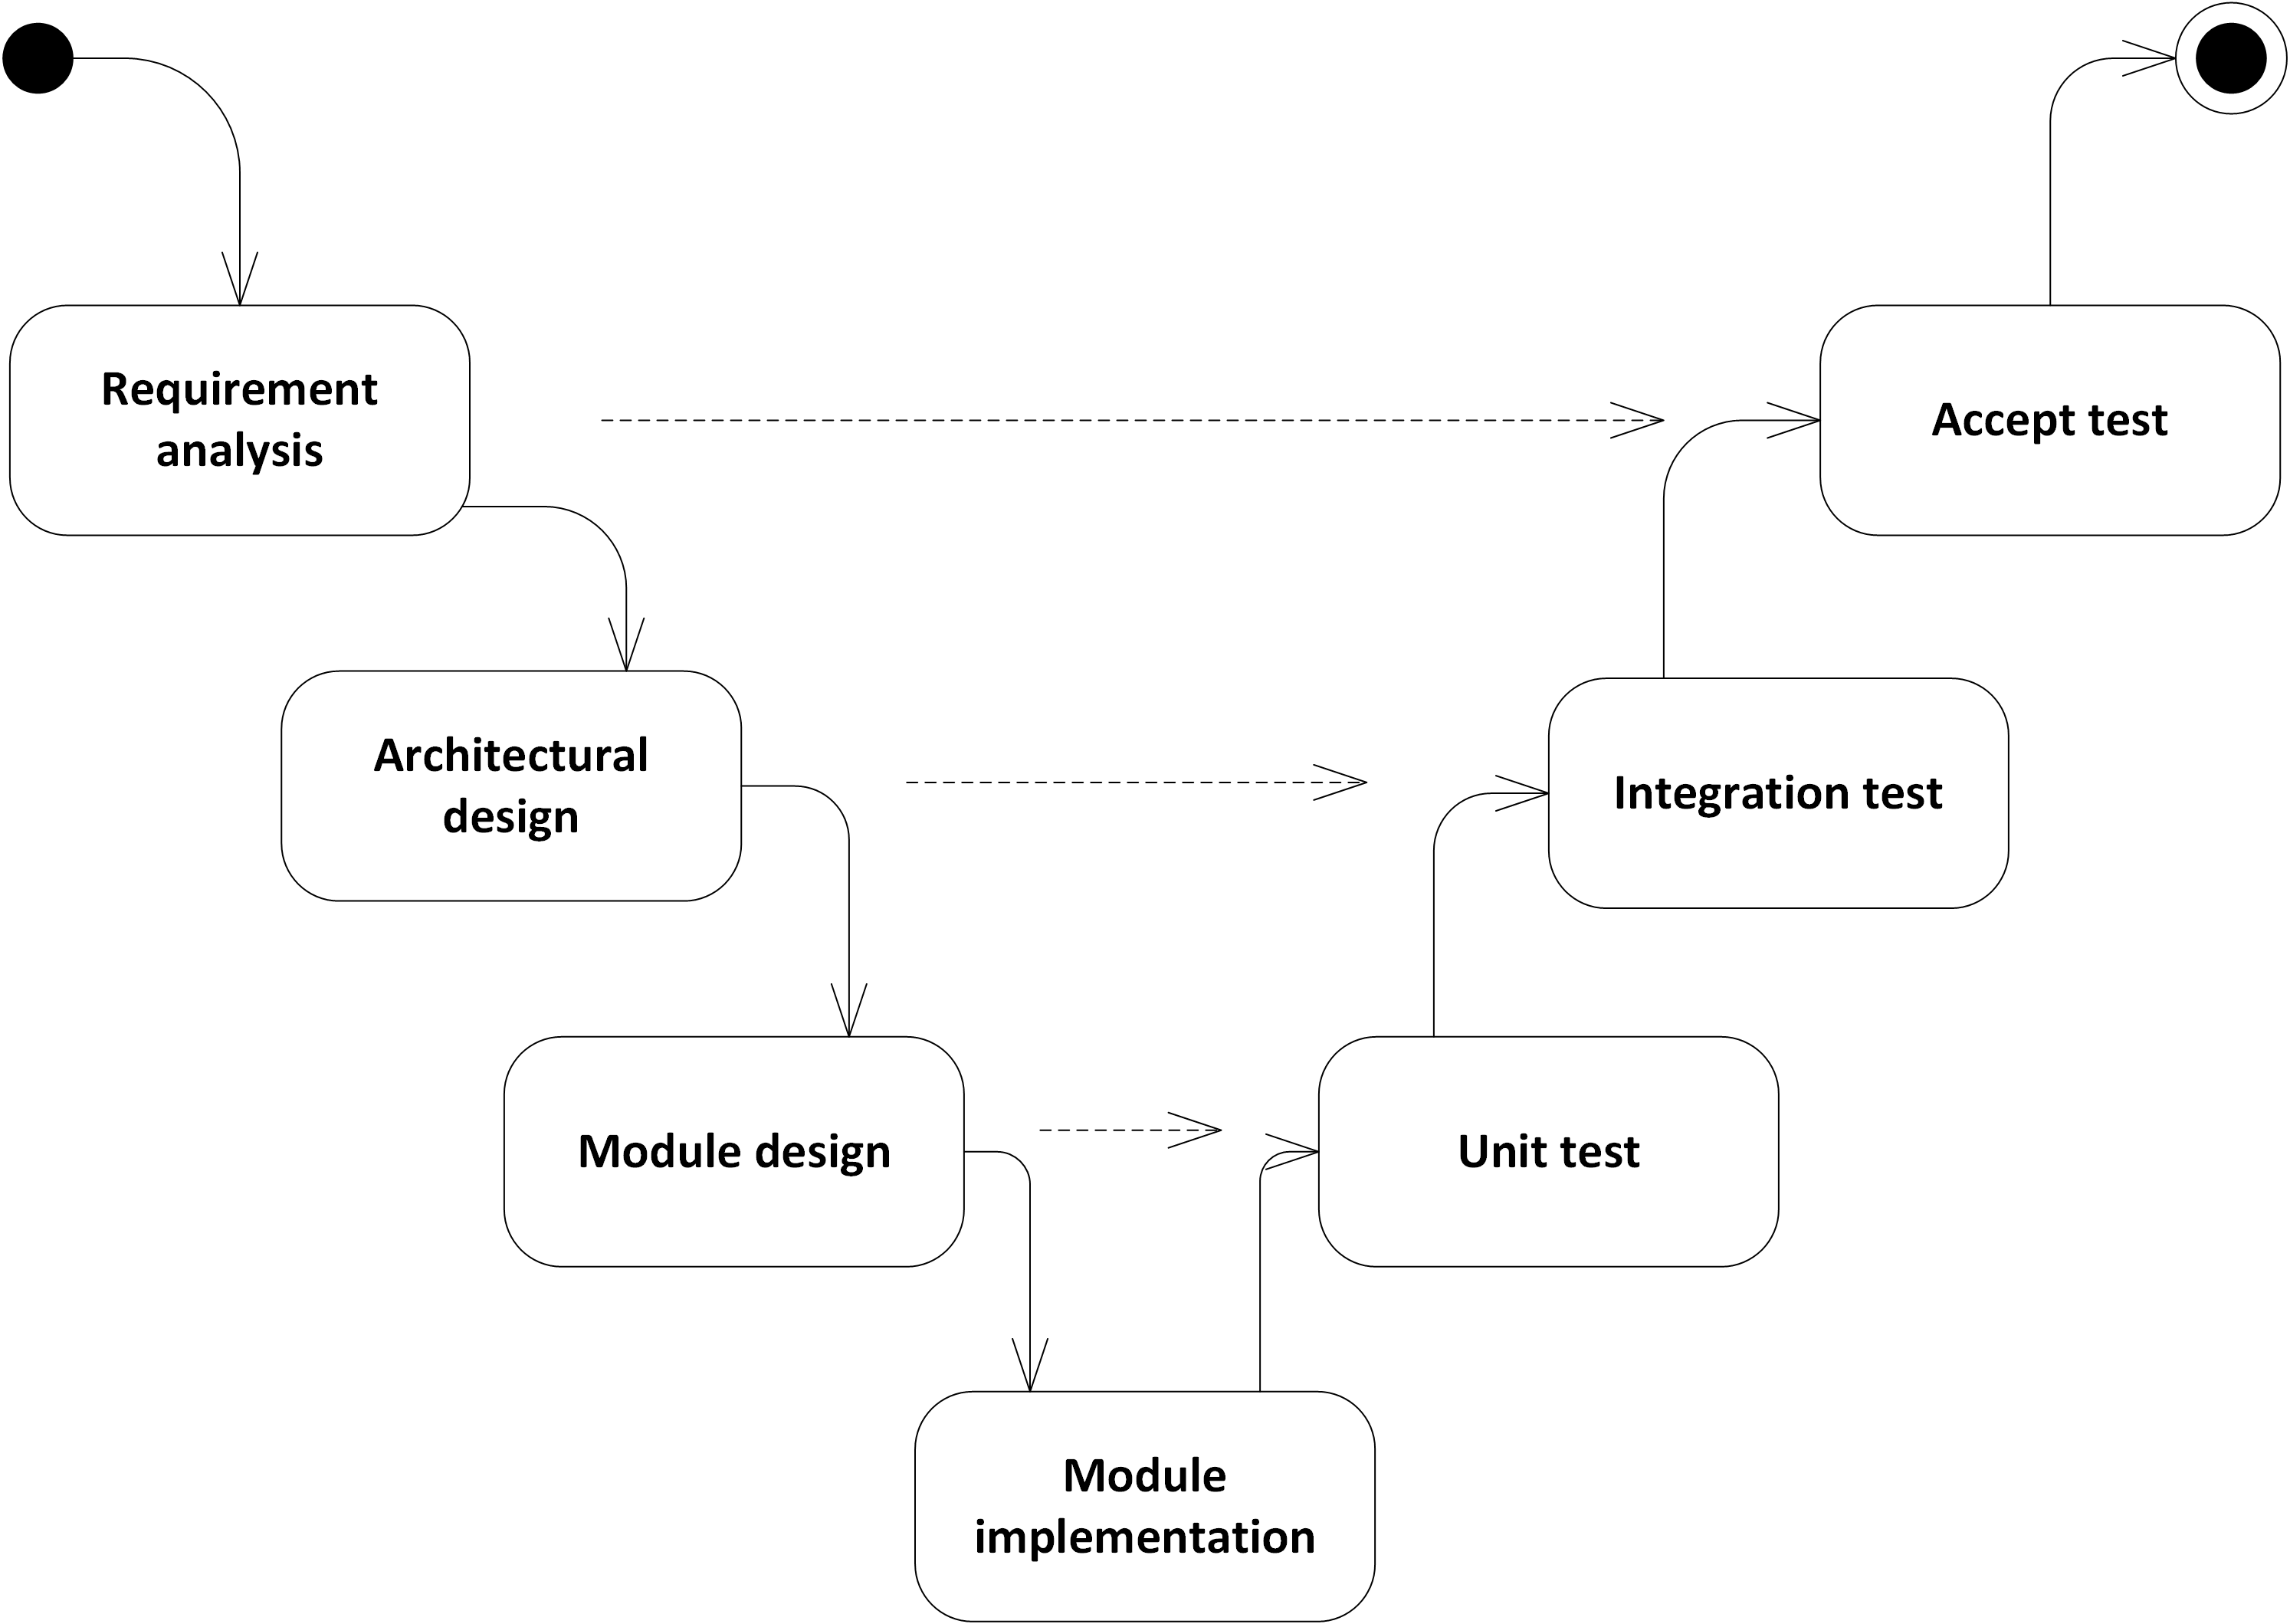
\includegraphics[scale=1.0]{Rapport/VModel.PNG}
	\caption{V-Modellen}
	\label{VModel}
\end{figure} 


\subsection{SCRUM}
Om end der måske ikke er blevet arbejdet fuld ud efter SCRUM principperne, har SCRUM haft stor betydning for hvordan arbejdet er blevet struktureret. I denne henseende har det været opbrydelsen af arbejdet i sprint og holdt daglige møder om arbejdet og opgaver. 
